\section{Preliminaries}\label{sec:prelim}

In this section, we give a brief description of Setchain and Tendermint being
the two basic blocks of this article.
%
For the sake of simplicity, we present just what we need from Tendermint to
implement Setchain on top of it.

\subsection{Setchain}
\setchain \cite{Capretto.2022.Setchain} is a distributed concurrent data-type
that implements Byzantine tolerant distributed grown-only sets with barriers
(called epochs).
%
Barriers impose an order between elements in different epochs but not with
elements in the same epoch.
%
Therefore, \setchain relaxes the total order requirement imposed by blockchains,
and thus, can achieve higher throughput and scalability.
%
\setchain can be used for those applications, like digital
registries, where different elements in the blockchain need not be
ordered except across infrequent barriers.

\paragraph*{Setchain API.}
%
Let \(U\) be a set of elements that client processes can inject into the
\setchain.
%
Moreover, let \isValidElement\ be a function that nodes can use to locally
validate elements in \(U\).
%
A \setchain is a distributed data structure where a collection of server nodes
maintain:
% \begin{compactitem}
\begin{itemize}
\item a set $\<theset> \subseteq U$ of elements added;
\item a natural number $\<epoch> \in \mathbb{N}$;
\item a map $\<history> : [1..\<epoch>] \rightarrow \mathcal{P}(U)$\footnote{$\mathcal{P}(U)$ denotes the
power set of $U$} describing sets of elements that have been stamped with an
epoch number.
\end{itemize}
%
Server nodes support two operations: \(\<add>\) and \(\<get>\).
%
Operation \(\<add>\) requests to add an element, while operation \(\<get>\)
returns the values maintained by the node~(\(\<theset>,\<history>,\<epoch>\)).
%
We use dot-notation to invoke these operations, let \(v\) be a server node and
\(e\) an element: \(v.\<add>(e),v.\<get>\).

% Each server node $v$ supports two operations,
% available to any client process:
% % \begin{compactitem}
% \begin{itemize}
% \item $v.\<add>(e)$: requests to add $e$ to $\<theset>$.
% \item $v.\<get>()$: returns the values of $\<theset>$, $\<history>$,
%   and $\<epoch>$, as perceived by $v$.
% \end{itemize}

When barriers are triggered, nodes maintaining the \setchain collaboratively
decide which added elements are stamped with the current epoch and increase the
epoch number.
%
We call these events \emph{epoch increments}.
%
We assume that periodic synchronization barriers are triggered.

A typical workflow from the point of the view of a client is as follows: a
client invokes $\<add>(e)$ in one (or more) servers to insert a new valid
element $e$ in the \setchain.
%
The element $e$ will be propagated among the servers, and when an
epoch increment occurs, the servers will attempt to include it in the
new epoch.
%
After waiting for some time, the client invokes $\<get>$ in one (or
more) servers to check that the element has been effectively added and
stamped.

\paragraph*{Properties.}
To ensure correctness, \setchain implementations must satisfy certain
properties that provide eventual guarantees for elements added and
guarantee consistency between correct servers. 
%
These properties reason about correct servers since Byzantine servers
do not provide any guarantee.

\begin{compactitem}
  \item Every valid element added by a correct
server is eventually returned in all future gets issued in all correct
servers.
  \item All valid elements added in a correct server must be eventually
be stamped in all correct servers.
  \item Once an element is stamped with an epoch, it cannot be unstamped, nor
can it be stamped with another epoch.
\item Any two correct servers agree on the content of
all epochs that both have computed~\footnote{Not all correct servers process epoch increments
simultaneously, as some may be more delayed than others.}.
%
% Nevertheless,
\item Every element that is stamped comes from the result of a client adding the element.
  \end{compactitem}
\gabina{Epoch proofs are part of the epoch but are not coming directly from the result of a client adding element.}

\subsection{Tendermint}\label{sec:tendermint}
%
Tendermint is a state machine replication engine that tolerates Byzantine faults.
%
It was among the first systems to adapt classical Byzantine Fault Tolerant consensus protocols
to the blockchain paradigm, whereby consensus is performed on cryptographic hash-linked batches of
transactions (i.e., blocks) in a public, open-membership network.
%
Tendermint functions as a blockchain middleware that supports the replication of arbitrary
applications, written in any programming language~\cite{tendermint.design}.

In Figure~\ref{fig:replication}, we show the overview of replicated state machine architecture.
%
A replicated state machine replicates a transaction log and resulting state across multiple machines.
%
Transactions are received from the client, run through the consensus protocol, ordered in the
transaction log, and executed against the state.
%
% In the figure, each , with .
%

\begin{figure}
  \centering
  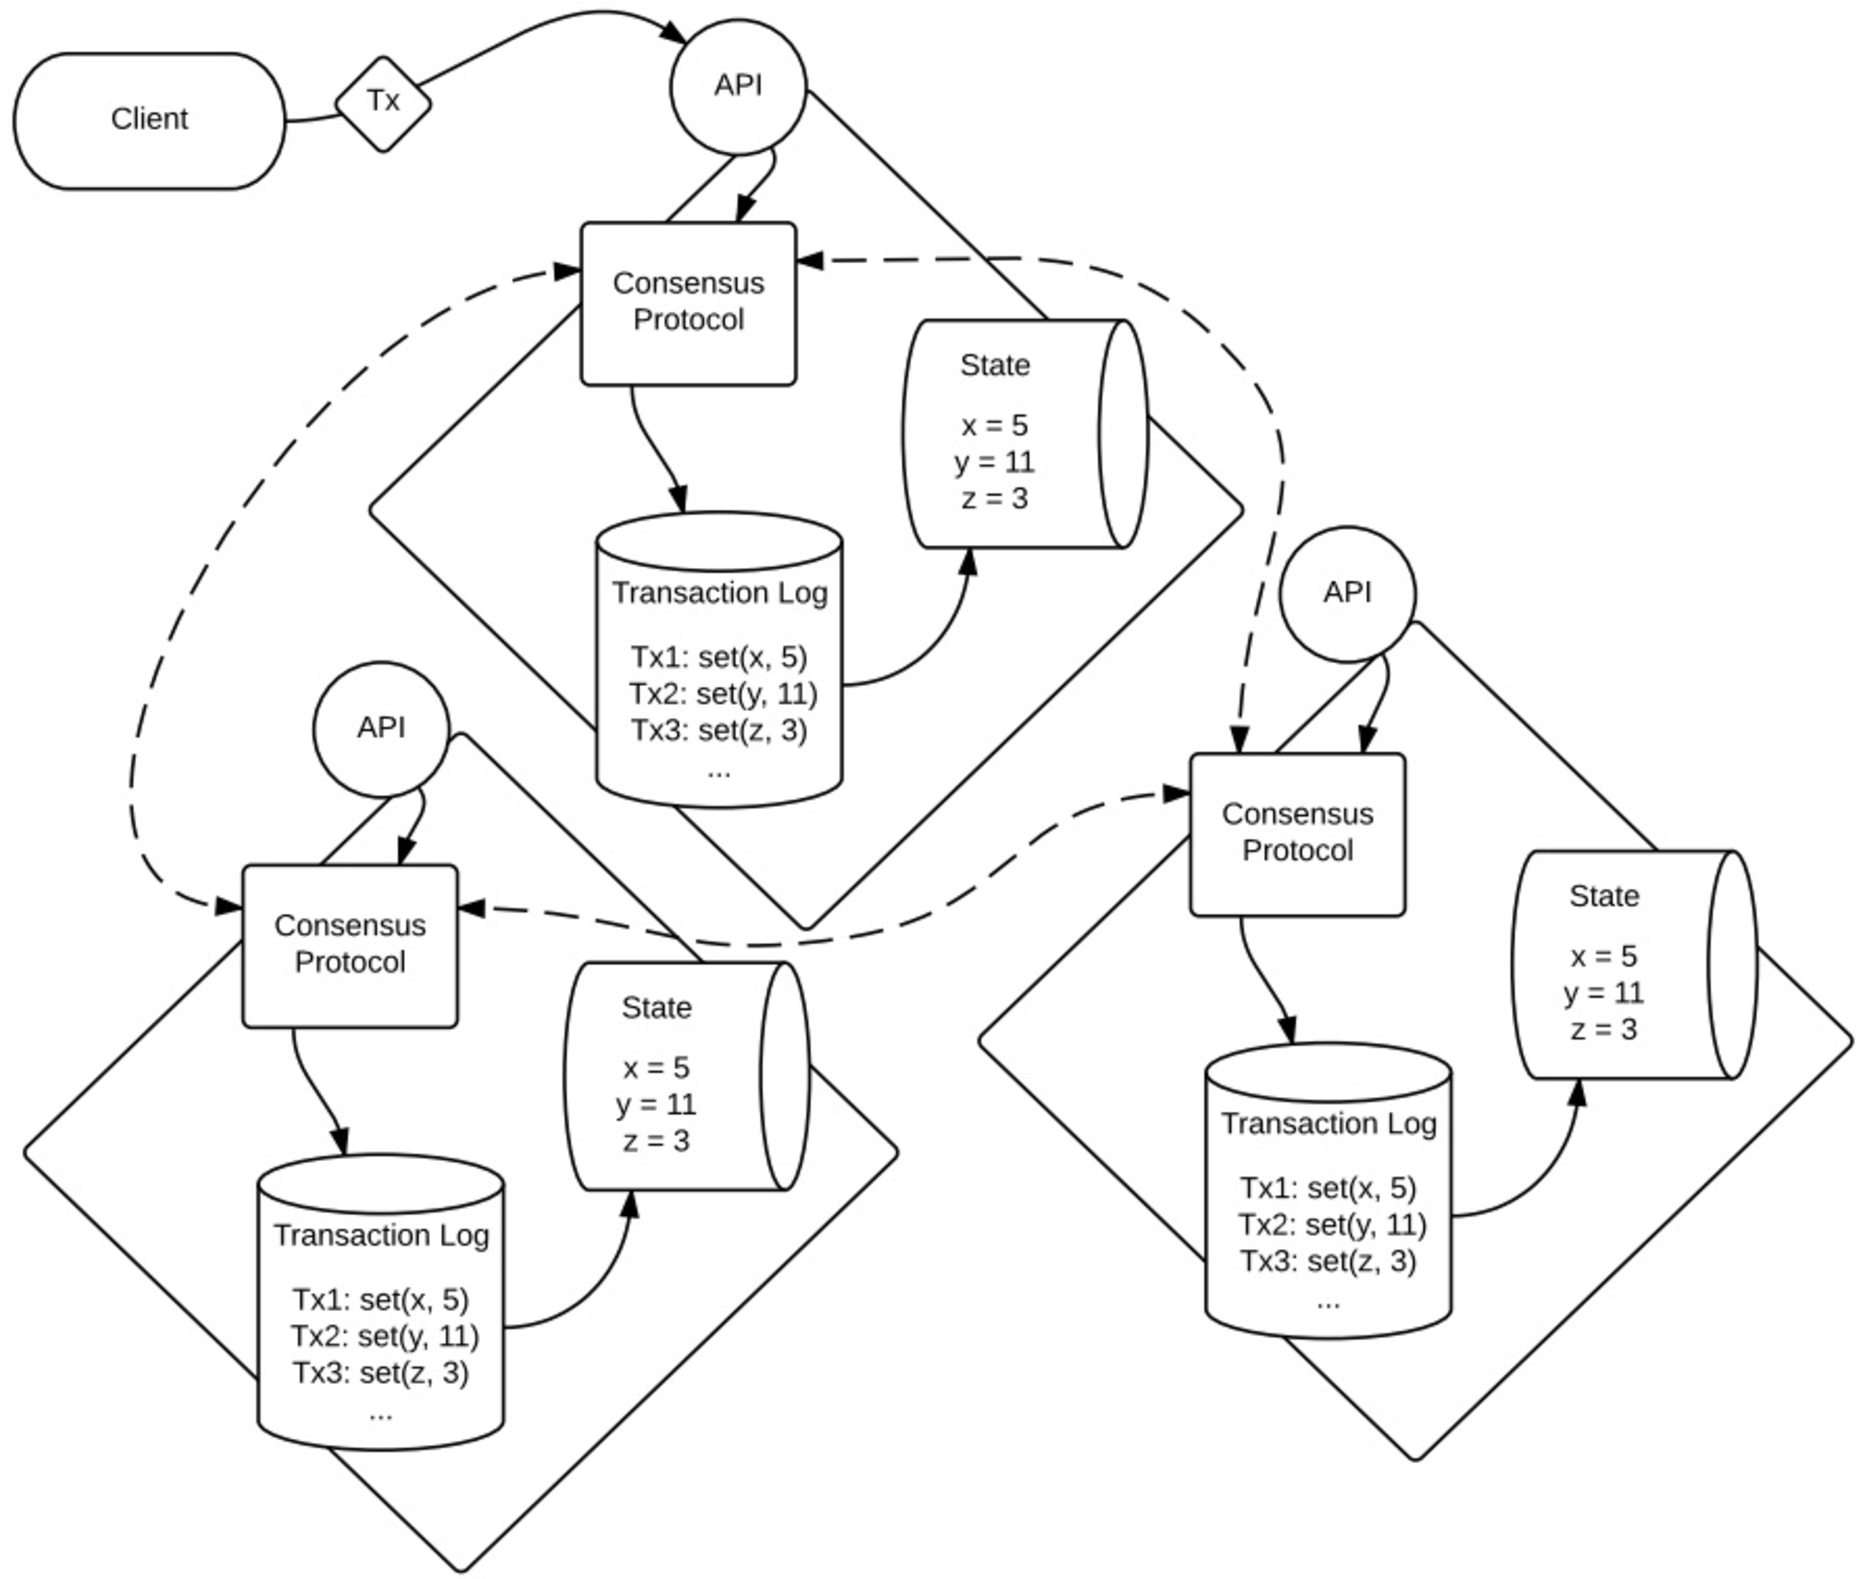
\includegraphics[scale=0.25]{figures/replication_engine.pdf}
  \caption{Overview of replicated state machine architecture~\cite{Buchman.2018.Tendermint}.
    %
    Diamonds represent machines.
    %
    Dotted lines represent communication between machines to carry out the
consensus protocol for ordering transactions
  }
  \label{fig:replication}
\end{figure}

%

Tendermint consists of two chief technical components: a blockchain consensus engine and a
generic application interface.
%
The consensus engine, called Tendermint Core, ensures that the same transactions are recorded
on every machine in the same order.
%
The application interface, called the Application BlockChain Interface (ABCI), enables the
transactions to be processed in any programming language.
%

\subsubsection{Application BlockChain Interface}
ABCI is the interface between Tendermint Core
% (the \textquotedblleft
% consensus engine\textquotedblright)
and the replicated application.
%
A Tendermint node maintains three main ABCI connections with the replicated application.
%

The \textit{consensus connection} is used only when a new block is committed,
and communicates all information from the block in a series of 
requests: \<BeginBlock>, [\<DeliverTx>, ...], \<EndBlock>, \<Commit>.
%
That is, when a block is committed in the consensus, Tendermint sends a 
list of \<DeliverTx> requests (one for each transaction) sandwiched by 
\<BeginBlock> and \<EndBlock> requests, and followed by a \<Commit>.

%

The \textit{mempool connection} is used by the transaction
pool protocol to validate transactions submitted
by clients against the application state. 
%
It is used only for \<CheckTx> requests. Transactions
are run using \<CheckTx> in the same order they were received
by the validator\footnote{Validator nodes are responsible for committing new blocks in the blockchain. These validators participate in the consensus protocol by broadcasting votes which contain cryptographic signatures signed by each validator's private key.}. If the \<CheckTx> returns OK, the transaction
is kept in memory and relayed to other peers in the same order
it was received. Otherwise, it is discarded.
%
It is up to the application to define whether a transaction is valid or not, and
the validation is optional. 

%

The \textit{query connection} allows retrieving information
from the local instance of the application, used by several
Tendermint modules (e.g., peer filtering).
%
It is used to query the application without engaging consensus. 
%It is exposed over the tendermint core rpc, so clients can query
%the app without exposing a server on the app itself.

Figure~\ref{fig:abci_flow} shows the flow of messages via consensus and mempool connections.
%

\begin{figure}
  \centering
  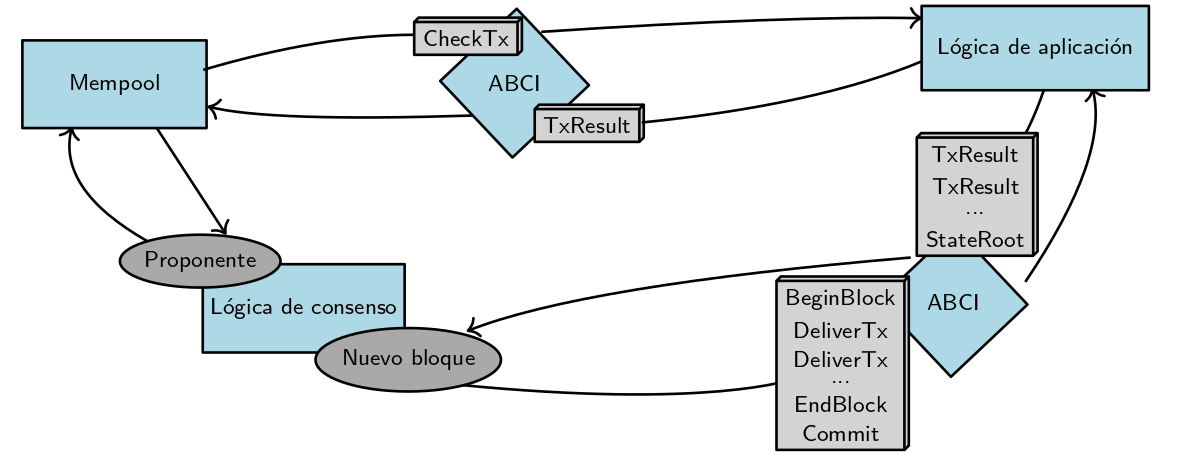
\includegraphics[scale=0.35]{figures/abci_msg_flow.pdf}
  \caption{Flow of messages via ABCI~\cite{tendermint.site}.}
  \label{fig:abci_flow}
\end{figure}

%%% Local Variables:
%%% TeX-master: "article.tex"
%%% TeX-PDF-mode: t
%%% End:
